\documentclass{article}
\usepackage{amsmath}
\usepackage{graphicx} % gráficos
\usepackage[noblocks]{authblk}
%\usepackage{float}
%\usepackage{cite}% para contraer referencias
%\usepackage[usenames]{color}
\usepackage{bm}
\newcommand{\abs}[1]{\lvert#1\rvert}
\usepackage{xcolor}
\newcommand{\notaL}[1]{{\color{blue}+L:#1+}}
\title{\textbf{Optimization of Porous Silicon Gradient Refractive
    Index Structures.} }
% A comparison with computational schemes with experimental results
\author[1]{C. A. Ospina de la Cruz}
\author[2]{W. L. Mochán }
\author[3]{V. Agarwal }

\affil[1]{Posgrado en Ingenier\'ia y Ciencias Aplicadas del Centro de
  Investigación en Ingenier\'ia y Ciencias Aplicadas (CIICAp-IICBA),
  Universidad Autónoma del Estado de Morelos (UAEM), Cuernavaca CP
  62209, México}
\affil[2]{Instituto de Ciencias F\'isica ,Universidad Nacional
  Autonoma de Mexico, Av. Universidad S/N, Col. Chamilpa, 62210
  Cuernavaca, Morelos, Mexico}
\affil[3]{Centro de Investigaci\'on en Ingenier\'ia y Ciencias
  Aplicadas,Universidad del Estado de Morelos, Av. Universidad 1001
  Col. Chamilpa, Cuernavaca, Morelos 62209, Mexico  }
\begin{document}

\maketitle
\notaL{Quité los intentos de tipografiar. Que de eso se encargue la
  revista.}
\notaL{Cambié la codificación a utf8; ya no uses latin1, es obsoleto.}
\notaL{Quité las líneas kilométricas. No te ocupes de su longitud y no
  juntes mis líneas.}
\notaL{Quité paquetes no escenciales}
\notaL{Cuida de no poner espacios al final de las líneas.}

\begin{abstract}
We propose a simple setup which allows the calculation of the current
density as a function of position within an electrochemical cell used
to produce porous Silicon structures with a controlled gradient in their
index of refraction. We produced samples under several conditions and
characterized them with scanning electron microscopy, and
ultraviolet-visible-near infrared reflectance spectroscopy. Our
results allow us to obtain from experiments on a single or just a few
samples a full characterization of the dependence of porosity,
dielectric function and speed of attack on the current density and on
position, so that novel nonhomogeneous devices may be designed and
built.

Keywords: Porous Silicon; GRIN; Reflectance Spectra.
\end{abstract}
\notaL{Cambié el abstract, pero habrá que revisarlo después.}
\section{Introduction}

\notaL{No entiendo nada de la introducción}
The structural properties of nanostructured materials  has  received a
considerable attention,  and a large research effort has been devoted
to them \cite{I1}. We found a great way to go for future
technological  explorations,  countless  challenges and  that  open a
range of possibilities to develop further  study  on these
issues\cite{I2}. Porous silicon (PS) is a versatile nanostructured
material and an excellent candidate as a technological platform for
different sensing applications \cite{I3, I4}, due to its easy
manufacturing,  large surface area, high surface reactivity,  and
moreover, its optical transduction capacity.  Photonic crystals are
multilayer dielectric structures that have periodicity in the
dielectric function along one direction \cite{I5}. It has numerous
studies for high reflectivity and the ability to adjust  the photonic
prohibited  band (PBG)\cite{I6} , which leads to possible applications
such as filters\cite{I7}, optical switches\cite{I8}, omnidirectional
mirrors\cite{I9}, waveguides for PC \cite{I10} etc. In the
conventional manufacturing of PS the desired result  is to obtain
homogeneous samples (same structural characteristics) from the
periphery  to the center  of the electrochemically  attacked area.
However, with an asymmetric anodizing configuration,  samples with a
lateral gradient in terms of pore size and thickness of the porous
layer are obtained \cite{I101}. In this configuration,  the face of
the platinum  electrode (cathode)  is relatively maintained
perpendicular  to the surface of the Si substrate (anode) at one end
of the cell, so that the distribution of the current within the
electrolyte  solution varies depending on the distance  of the
electrode due to the resistance of the electrolyte,  resulting  in a
decrease in current density as the distance from the electrode
increases \cite{I102, I103}. The result is a porous surface with
different pore sizes ranging from a few nanometers  to pores on the
order of a few micrometers  \cite{I104}. The dimensions of the pores
obtained on the same chip can be controlled by adjusting the anodizing
current and electrolyte concentration \cite{I11}. Currently, these
types of samples have found their application relevant as optical band
filters \cite{I12}, devices with a multidirectional photonic band
(photonic bar codes) \cite{I13} and mainly as biosensors. In this way,
the effect of different topographies (porosities in the same sample)
on the culture / adhesion of certain cells \cite{I14} is studied,
considerably reducing the number of samples and cost of the study. In
addition, they are also very useful when a biomolecule size-exclusion
technique is required allowing the identification and separation of
these biological compounds \cite{I15}. Recent studies  have shown that
the  combination  of thermal  oxidation  and infiltration of TiO2   by
ALD offers the  opportunity to manufacture  a high index of refraction
of contrast, visibly transparent GRIN optical elements from PS
absorbent structures \cite{I16}. A Despite previous research on the
formation of porous silicon with GRIN, type p in manufacturing and
characterization, there was no control of current densities, much less
a model that  explained said lateral  gradient. In this work, we
reported a gradient refractive index (GRIN) structure by varying the
current density on the fabrication of porous silicon photonic
structure. This current density values, depth, and porosity of the
photonic structure were calculated from an electrostatic model for
photonic crystals with a gradient refractive index
(EMPCGRIN). Moreover, the theoretical and experimental studies were
exhibited similar results.

The paper is organized as follows. In Section 2  we report the effect
of how the current density can be calculated from an electrostatic
model for photonic crystals with gradient refractive index (EMPCGRIN),
demonstrating that there is a direct relation of the gradient
generated by the electrode when it attacks the Silicon sample, we can
see the depth of the structure and its porosity, in each of the
measuring points. In Subsection 2.2 we present a formalism based on
the methods used for the analysis of photonic crystal structures is
the transfer matrix method. We use it to investigate the reflectance
of light in a one-dimensional photonic crystal. In Section 3 we
provide experimental  details about the manufacture of PS dielectric
multilayers and Section 4 we shows the comparison of numerical and
experimental results followed. Finally,  the conclusions given in
Section. 5

\section{Theory}
\subsection{Calculation of the current density}
\notaL{check where acronyms are first defined}
A gradient in the optical properties of porous Silicon (PS) systems may be
obtained by electrochemically attacking a Si surface with a position dependent current
density ${\bm j(\bm r)}$, as the porosity and refractive index depend on
the current density, as well as the speed of attack and the width of the
porous layer. Nevertheless, it is not a simple to task to measure the
{\em local} value of $\bm j(\bm r)$ along the surface. This hampers the
design and optimization of well characterized reproducible GRIN PS
structures. Thus, a system for which the current density field may be
easily computed would be useful.
Though $\bm j(\bm r)$ may be in principle be numerically calculated for a
given arbitrary experimental setup,  here we propose a particularly
simple setup that allows an expression for the current in terms
of a series that is rapidly convergent and each of whose terms is a
simple analytic function. With this setup it is easy to characterize
the dependence of different properties of interest on the current, and
this allows the design and optimization of diverse GRIN PS devices.

We assume that our electrolytic cell has the shape of a
prism (see Fig. \ref{f:celda}) with a horizontal rectangular base of sides $a$ and $b$, and
filled with the electrolyte up to a height $c$. We assume that the
walls of the cell are insulating while the bottom is completely
covered with the sample, which is a good conductor which is
electrically grounded. Within the electrolyte we position an electrode
which we assume is a thin conductor, insulated from the electrolyte
but for a small area near its tip, which we thus approximate as a
point current source.
\begin{figure}
  \centering
  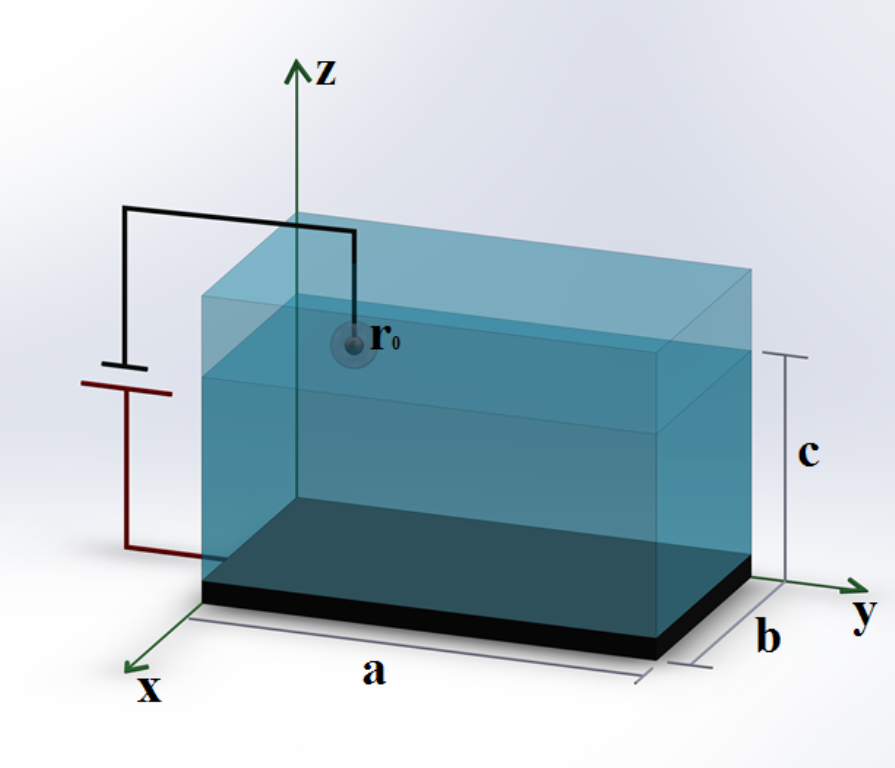
\includegraphics[scale=.4]{Images/celdan}
  \caption{Prism shaped electrolytic cell with a rectangular base of
    sides $a$, $b$ filled with electrolyte up to a height $c$. The
    walls of the cell are insulating and the bottom is completely
    covered by the sample, which is assumed to be a good
    conductor. The tip of the electrode is a thin insulated wire with
    just the tip uncovered and located at $ \vec{r}_0 $ within the
    liquid.\notaL{Quité el tipo de letra del pie de figura. Que la pongan en la
      revista.}\notaL{En la punta pusiste dos esferas. Quítalas y sólo
    pon un puntito dorado del ancho del cable. Muestra que la base
    está aterrizada}\notaL{Indica el voltaje y la
    corriente}\notaL{¿Está bien la polaridad de la batería?}}
  \label{f:celda}
\end{figure}
Within the electrolyte the current density is
\begin{equation}
  \label{eq:j}
  \bm j=\sigma\bm E,
\end{equation}
with
$\sigma$ the conductivity, $\bm E=-\nabla\varphi$ the electric field,
and $\varphi$ the electric potential. For a
stationary situation\notaL{Latex usa nabla como el nombre de
  $\nabla$}
$\nabla\cdot \bm j = \sigma\nabla\cdot\bm E=0$. Thus, within the electrolyte,
\begin{equation}
  \label{eq:laplace}
\nabla^{2} \varphi=0.
\end{equation}
Consider now an arbitrary closed surface
$\mathcal S$
within the electrolyte that surrounds completely the tip of the
electrode. Integrating $ \bm j$ over this surface we obtain
\begin{equation}
  \label{eq:I}
\int_{\mathcal S'} d\bm a \cdot \bm j = I,
\end{equation}
where the prime on $\mathcal S'$ means we remove from the surface a
very small hole through which the wire that feeds the current gets
through. Assuming the wire is narrower than any other relevant
distance in the system, we may interpret Eq. \eqref{eq:I} as an
integral over a closed surface of the current \eqref{eq:j} within the
electrolyte, ignoring the actual current within the wire. Thus
\begin{equation}
  \label{eq:gauss}
  \int_{\mathcal S} d\bm a \cdot \bm E = \frac{I}{\sigma}
\end{equation}
Using Gauss's law, we interpret this equation as a source for the
potential in the form of a point charge
\begin{equation}
  q_{_{0}} = \frac{I}{4 \pi \sigma}
\end{equation}
at the position $\vec{r}_{_{0}}=(x_{_{0}}, y_{_{0}}, z_{_{0}})$ of the
tip of the electrode. Note that $q_0$ would be the total charge,
and it shouldn't be further screened through the permittivity of the
electrolyte.

The effective conductivity of the relatively thin sample in contact
with the grounded counterelectrode is large enough that we may assume its
surface $z=0$ is an equipotential.
On the other hand, no current can go across the insulating walls of
the cell, situated at $x=0$, $x=a$,, $y=0$ and $y=b$, nor through the
free surface of the liquid at $z=c$. Thus, the problem to solve is Poisson's
equation with a point charge source
\begin{equation}
  \label{eq:poisson}
  \nabla^2\varphi=-4\pi q_0\delta(\bm r-\bm r_0),
\end{equation}
with mixed boundary conditions
\begin{equation}
  \label{eq:ground}
  \varphi(x,y,0)=0,
\end{equation}
and
\begin{equation}
E_{_{x}}(0, y ,z)= E_{_{x}}(a, y ,z)=E_{{_y}}(x, 0 ,z)=E_{{_y}}(x, b
,z)=E_{{_z}}(x, y ,c)=0.
\end{equation}
This problem may be solved readily using image charge theory
\notaL{ref}. The potential within the electrolytic cell coincides the
the field within an infinite vacuum containing the point charge
$q_0$ at the tip of the electrode at $\bm r_0$, and an array of its fictitious image
charges. The images include a reflection on the conducting bottom of the
cell, of the opposite charge $-q_0$ and situated at $(x_0, y_0,-z_0)$,
to guarantee that the bottom stays at potential zero.
There are further images on the four walls of the cell, of the same charge $q_0$
and situated at $(-x_0,Y_0,z_0)$, $(x_0,-y_0, z_0)$, $(2a-x_0, y_0,
z_0)$ and $(x_0, 2b-y_0,z_0)$ to guarantee that no current goes across
them. Similarly, there is an image of the same charge $q_0$ at
$(x_0,y_0,2c-z_0)$ to guarantee that no current goes across the
surface of the electrolyte. Furthermore, each image charge has to be
further reflected by each of the aforementioned surfaces, yielding new
images.
\begin{figure}
  \centering
  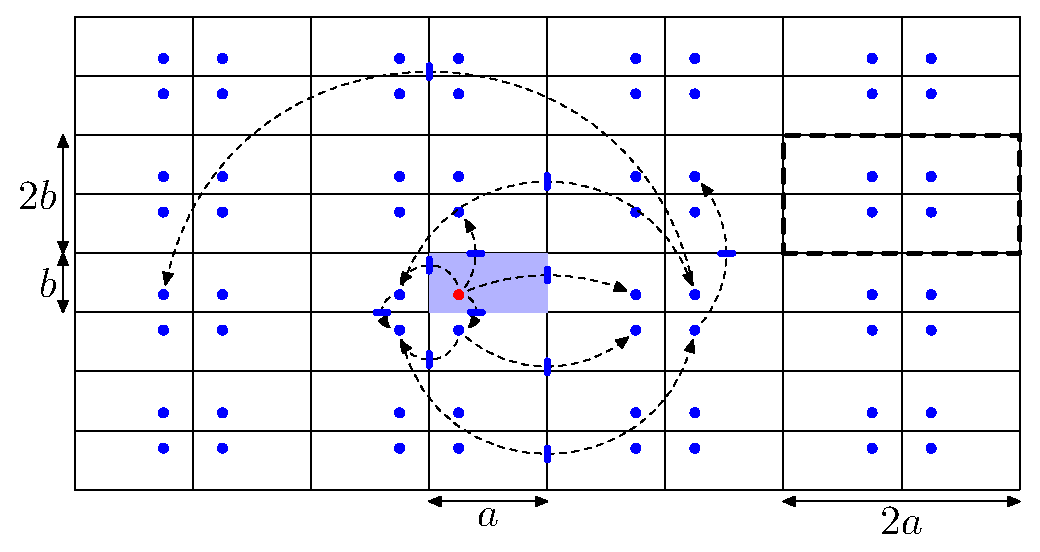
\includegraphics[width=\textwidth]{paper-1}
  \caption{Top view of the electrolytic cell (light blue) showing the charge at the
    tip of the electrode (red dot) and its images on the walls of the
    rectangular cell, the images of its images and so on (blue dots). The walls are at $x=0,a$,
    $y=0,b$. The relation of some charges and their images is
    indicated by dashed arrows, with a bar to indicate the
    corresponding reflecting wall. The system may be interpreted as a
    periodic lattice with a rectangular unit cell of size $2a\times 2b$,
    one of which is indicated  by wide dashed lines, and with a basis of four equal
    charges at $(\pm x_0, \pm y_0, z_0)$.}
  \label{fig:topview}
\end{figure}
In Fig. \ref{fig:topview} we illustrate the real charge and all of
its images within the plane $z=z_0$. They form a periodic rectangular
lattice with a unit cell of size $2a\times 2b$ and with a basis of
four equal charges situated at the positions $\bm r_0$, $\bm
r_1=(-x_0, y_0, z_0)$, $\bm r_2=(x_0, -y_0, z_0)$ and $\bm r_3=(-x_0,
-y_0, z_0)$. In Fig. \ref{fig:sideview} we show a lateral view of the
image charges.
\begin{figure}
  \centering
  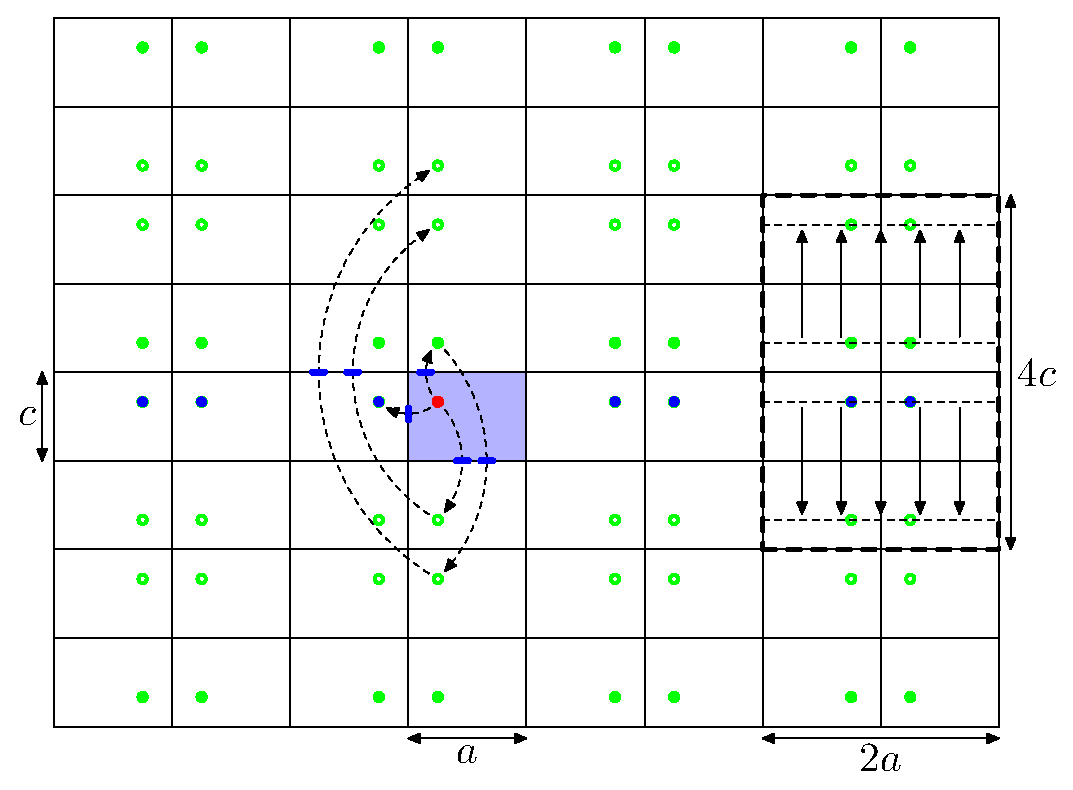
\includegraphics[width=\textwidth]{paper-2}
  \caption{Side view of the electrolytic cell (light blue)
    showing the charge at the tip of the electrode (red dot), its
    images within the plane $z=z_0$ (blue dots), and its images at the
    surface of the sample and the top of the electrolyte (green
    dots). We use solid dots to denote particles with the same charge
    as that corresponding to the tip $q_0$, and open dots for those of
    opposite charge. The system may be interpreted as a periodic
    lattice with a rectangular unit cell of size $2a\times 4c$, one of
    which is indicated by wide dashed lines, and with a basis of four
    charges $q_0$ and another four charges $-q_0$. Within this cell,
    we indicate its $G=0$ contribution to the electric field (solid
    arrows, see text).}
  \label{fig:sideview}
\end{figure}
Each plane of charges upon reflection on the surface of the sample yields an
plane of image charges of the opposite sign, while reflections
on the surface of the liquid yields a plane of charges of the same
sign. The side view may be interpreted as a periodic rectangular
lattice with a unit cell of size $2a\times 4c$ containing a basis of eight point
charges, four positive and four negative. A projection onto the $yz$
plane would similarly yield a rectangular lattice with a  $2b\times4c$
unit cell. Putting everything together, the problem is that of solving
Poisson's equation within an orthothombic lattice of size
$2a\times2b\times4c$ with a basis of 16 point charges of charge $\pm
q_0$ arranged in positive and negative planes.

The electrostatic potential produced by an infinite array of
charges expressed as a sum in real space of Coulomb terms has ill
convergence properties. The potential can be obtained
using the Ewald summation technique \notaL{ref}, which yields two rapidly converging
series, one in real space and another one in reciprocal space.
Nevertheless, as we need the potential and the field to obtain the
current density on the surface of the sample on which there are no
real nor image charges, we may perform a somewhat simpler planewise
summation, where we first obtain the potential and field produced by a
simple periodic lattice of charges using a fast convergent sum over the 2D
reciprocal vectors, and then sum over the charges that form the basis
of the 2D {\em crystal} plane and finally sum over all the planes \notaL{ref}.

We consider first a system made of identical unit charges
ocuppying the positions $\bm R$ of a 2D Bravais lattice $\{\bm R\}$,
which we will take as a rectangular lattice with lattice parameters
$2a$ and $2b$, and lying, for the time being, at the $z=0$ plane.
The potential it produces obeys
\begin{equation}
  \label{eq:poissonRed}
  \nabla^2\varphi(\bm r)=-4\pi\sum_{\bm R}\delta(\bm r_\|-\bm
  R)\delta(z)=-\frac{4\pi}{A}\sum_{\bm G}e^{i\bm G\cdot\bm r_\|}\delta(z),
\end{equation}
where $\bm r_\|$ is the projection of the observation position $\bm
r=(x,y,z)$ onto the $xy$ plane,
$\delta(\ldots)$ is Dirac's delta function, $\{\bm G\}$ is the
reciprocal lattice defined through $e^{i\bm G\cdot\bm R}=1$ for all
$\bm R$ and $\bm G$, $A=4ab$ is the area of the unit cell
and we used the Fourier representation of the 2D
periodically repeated delta function. We introduce a 2D Fourier representation for
the potential \notaL{Checar consistencia entre phi y varphi en todos lados}
\begin{equation}
  \label{eq:phifourier}
  \phi(\bm r)=\sum_{\bm G}\phi_{\bm G}(z)e^{i\bm G\cdot\bm r_\|}
\end{equation}
where $\phi_{\bm G}(z)$ is the Fourier coefficient of the potential at
the height $z$. Substitution in Eq. \eqref{eq:poissonRed} yields the
ordinary differential equation \notaL{El signo estaba mal. Chécalo.}
 \begin{eqnarray}
 \frac{d^2}{dz^2}\phi_{\bm G}(z)-G^2\phi_{_{G}}(z)=
   -\frac{4 \pi}{A} \delta(z),
 \end{eqnarray}
an homogeneous equation for $z\ne0$ which may be trivially
solved. After applying boundary conditions at $z=0$ and regularity
conditions at infinity, we obtain
\begin{equation}
  \label{eq:phiG}
  \phi_{\bm G}(z)=
  \begin{cases}
    -\dfrac{2\pi}{A}\abs{z}&\text{if }G=0,\\
    \dfrac{2 \pi}{AG}  e^{- G \abs{z}}&\text{if }G\neq 0.
  \end{cases}
\end{equation}
The case $G=0$ corresponds to the potential produced by a uniformly charged plane,
while the case $G\ne 0$ is the symmetric solution that decays far from
the source plane. Substituting into Eq. \eqref{eq:phifourier} yields
\begin{eqnarray}
  \label{eq:phiG1}
 \phi(\bm r) = -\frac{2 \pi}{A}  \abs{z} +{\sum_{\bm G}}' \frac{2 \pi
   }{AG} e^{- G \abs{z}} e^{i \bm G\cdot\bm r_\|},
 \end{eqnarray}
where the prime indicates that the term $G=0$ should be ommited from
the sum.

We consider now the basis of our 2D lattice, with equal charges at the
four positions $(\pm x_0, \pm y_0)$. Each of the corresponding four
sublattices produces a potential as that in Eq. \eqref{eq:phiG1} but
shifted by the corresponding basis vector, yielding
\begin{equation}
  \label{eq:phiG4}
  \phi(\bm r) = -\frac{8\pi}{A} \abs{z}
    +{\sum_{\bm G}}' \frac{8\pi}{AG} e^{- G \abs{z}}\cos(G_x x_0)
    \cos(G_y y_0) e^{i \bm G\cdot\bm r_\|}.
\end{equation}
Finally, we shift the origin of Eq. \eqref{eq:phiG4} vertically to each of the planes shown in
Fig. \ref{fig:sideview} and multiply by the corresponding charge $q_0$
or $-q_0$ to obtain the contribution to the total potential. The charge $q_0$ corresponds to
the planes with heights of the form $z_0+4nc$ and $-z_0+(4n+2)c$, with
$n=\ldots-2,-1,0,1,2\ldots$ an arbitrary integer, while the charge
$-q_0$ corresponds to the planes with height $z_0+(4n+2)c$ and
$-z_0+(4n+4)c$.

We concentrate our attention only on the region $a\le z<z_0$. From
Fig. \ref{fig:sideview} we see that the $G=0$
field has contributions only from the charges at $z_0$ and their
images ant $-z_0$, this contribution is like that of a parallel plate
capacitor $E_{0z}=-4\pi q_0/ab=-16\pi q_0/A$, which corresponds to the
potential $\phi_0=16\pi q_0 z/A$. Other contiguous planes of with opposite charges
contribute to the field elsewhere. The contributions to the potential
from the $G\ne0$ are simple geometric sums that may be summed
analytically over $n$ and yield the total potential
\begin{equation}
  \label{eq:phitot}
  \begin{split}
    \phi(\bm r)=&\frac{16\pi q_0}{A}\biggl(z+{\sum_{\bm G}}'\frac{2\sinh
      Gc}{G \sinh 2Gc}\cosh G(c-z_0)\cos G_x x_0 \cos G_y y_0\\
    &\times \sinh Gz\, e^{i\bm G\cdot\bm r_\|}\biggr).
  \end{split}
\end{equation}

Notice that the terms of the sum above converge exponentially to zero
as $G$ increases for any $z$ such that $0\le z <z_0 \le c$, and thus
the sum is convergent. The divergence in the limit $ z
\longrightarrow z_0 $ is not worrisome, as we are interested in the
field close to bottom $z=0$ of the cell.

The current density normal to the surface may now be obtained as
$j_\perp=-\sigma\partial\phi/\partial z$,
\begin{equation}
  \label{Eq:J}
  \begin{split}
    j_\perp(\bm r) =& -\frac{I}{ab}\biggl(1+{\sum_{\bm G}}'\frac{2\sinh
      Gc}{\sinh 2Gc}\cosh G(c-z_0)\cos G_x x_0 \cos G_y y_0\\
    &\times \cosh Gz\, e^{i\bm G\cdot\bm r_\|}\biggr).
  \end{split}
\end{equation}
Eq. \eqref{Eq:J} is a very rapidly convergent expression that allows,
in particular, to calculate the current $j_\perp(x,y,0)$ that attacks
the substrate to produce the PS sample.
Integrating over the surface of the sample we verify
\begin{equation}
  \label{eq:intj}
  \int_0^adx\int_0^bdy\,j_\perp(\bm r)=-I,
\end{equation}
as the contributions of opposite non-null reciprocal vectors cancel
out. As expected, all of the current that leaves the electrode find
its way to the substrate.

Using Eq. \eqref{Eq:J} we can correlate the local current density at
the sample as it is prepared with its geometric and optical
properties. For the calculation of the optical properties we use the
well known transfer matrix method \notaL{refs}.

\section{Experimental Details}
\begin{figure}
  \centering
  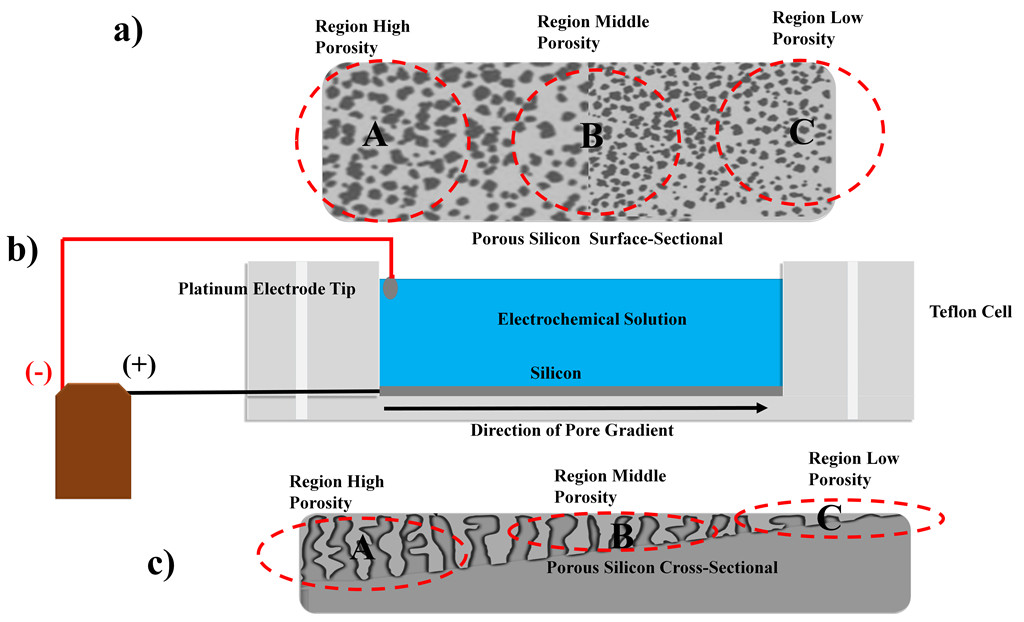
\includegraphics[scale=0.6]{Images/DE1}
\caption{\emph{Schematic of the experimental set-up for
      fabrication of porous silicon with GRIN. (a) Represents an
      outline of the surface section, divided by three regions
      A, B and C, corresponding to High, Medium and Low Porosity
      respectively. (b) It is the diagram of the electrochemical
      cell with its parts: silicon wafer, Teflon cell, platinum
      point electrode, Electrochemical Aqueous solution and the
      connection of the circuit with the cathode and anode. (c)
      It is a schematic drawing of the Cross section of the
      electrochemically attacked porous silicon seen in three
      different regions as mentioned above. }}
    \label{fig:DE1}
  \end{figure}

In the Fig. \ref{fig:DE1} a shows schematic representation of the
experimental setup where porous silicon can be manufactured with GRIN,
taking into account the considerations of the electrode as tip, the
rectangular cell and the sample (silicon wafer) with the largest
rectangular attack area.
In Fig. \ref{fig:DE1} a) we draw an outline of the surface section,
divided by three regions A, B and C, dependes in therir porosity i.e.,
High, Medium and Low Porosity. All this corresponding to  expected to
be obtained in the experiments. Fig. \ref{fig:DE1} b) the scheme shows
the electrochemical cell with its parts: silicon wafer, teflon cell,
platinum point electrode, electrochemical Aqueous Solution and the
connection of the circuit with the cathode and anode. Finally,
Fig. \ref{fig:DE1} c) it is a schematic drawing of the Cross section
of the electrochemically attacked porous silicon seen from three
different regions as mentioned above. In section 3.1 we give the
details used to carry out our experiments.

\subsection{Fabrication of Porous Silicon Monolayers GRIN}
Some of the simulated photonic structures were made by electrochemical
anodization on an oriented (100) p-type crystalline Si wafer
(resistivity 0.002 - 0.005 $ \Omega \cdot cm $), under galvanostatic
conditions. The electrochemical anodization process was performed at
room temperature, with an electrolytic mixture of aqueous hydrofluoric
acid (HF) (concentration: 48 $ \% $ wt), glycerol (purity: 99.8 $ \% $
wt) and ethanol (purity: 99.9 $ \%$ wt ) in 3: 7: 1 volume ratio,
respectively. After the anodizing process, the samples are rinsed with
ethanol (purity: 99.9 $ \% $  wt). The layout of the cell used is as
seen in Fig. \ref{fig:DE1} b), with an area of $ 1,206 \ \ cm^2 $
(this is the area attacked in the process), has a rectangular shape ($
0.62 \ \ cm \times 2.03 \ \ cm $)  so that the current densities  that
attacks has a lateral gradient with a greater surface area. They were
manufactured with a fixed current of $ 5 \ \ mA $ to generate
different current densities ranging from $ 6  $ to $ 2.5 \ \ mA / cm^2
$. Similarly, we use the current from $ 40 \ \ mA $ to generate $ 50 $
to $ 20 \ \ mA / cm ^ 2 $. The cathode is made of a platinum wire that
was arranged in the form of a tip with an approximate diameter of ($
0.5 \ \ mm $).
\subsection{Reflectance Measurement}
In the experiemental parte the reflectivity measurements were carried
out with a Perkin Elmer Lambda 950 UV-Vis-NIR spectrophotometer. To
calculate the complex refractive index $ \tilde{n}_{_{PS}} = n_{_
  {PS}} - ik_{_{PS}} $ of a porous layer with homogeneous porosity
and thickness with smooth interfaces to throughout the entire
structure, the more suitable is the adjustment procedure of the
experimental reflectance or transmittance spectrum, this is for the
theoretical part. In the case of the reflectance spectrum. The
corresponding theoretical calculations were carried using procedure
for single  smooth layer (monolayer).
 \begin{eqnarray}\label{Eq:ECMR}
R=\dfrac{r _ {_ {01}}r _ {_ {12}} e^{-2i\delta}}{1+r _ {_ {01}}r _ {_ {12}} e^{-2i\delta}}
\end{eqnarray}
where $ r_{_ {01}} $ y $ r_{_ {12}} $ are the Fresnel reflectance
coefficients at the interfaces $aire/PS$ y $PS/c-Si$ which are
defined in terms of their complex refractive index ($\tilde{n}_{_ {1}}
$, $\tilde{n}_{_ {2}} $ y $ \tilde{n}_{_ {3}} $), for them
$r_{_{ij}}=(\tilde{n}_{_{i}}\cos\theta_i-\tilde{n}_{_{j}}\cos\theta_j)/(\tilde{n}_{_{i}}\cos\theta_i+\tilde{n}_{_{j}}\cos\theta_j)$,
($j=i=0,1,2$), whilst $\delta=2\pi
d/\lambda\sqrt{\tilde{n}^2_{_{2}}-\tilde{n}^2_{_{1}}\sin \theta_1}$.
 To adjust the reflectance spectrum, the layer thickness is an input
 parameter in the Eq.\ref{Eq:ECMR}. The advantage of this method is
 the possibility of taking into account the interface roughness effect
 by including the Davies-Bennett factor in the coefficient of each
 Fresnel \cite{I17, I18, I19}, which represents the roughness of a
 Gaussian distribution.
\subsection{Morphological studies}
The morphologies of the etched porous layers (cross-sectional) was
observed using SEM Hitachi SU1510 scanning electron microscopes
(Hitachi High Technologies Canada, Inc., Toronto, Canada), the
thickness  and porosity  of each fabricated  film was measured.
 \subsection{Refraction Indices Monolayer of Porous Silicon GRIN }
Through the electrochemical anodization of c-Si wafers, Psi monolayers
were obtained. For the refractive index of each monolayer Psi
calcalated by ussing  Bruggeman effective medium theory, as we
consider that we have a homogeneous medium associated with effective
dielectric function \cite{I20}. This effective dielectric function is
related to the dielectric functions of the two media, consisting of
two materials (air and silicon), where it is assumed that all the
pores or islands of the bulk material experience an average electric
field; the equation is expressed as follows:
 \begin{eqnarray}\label{Eq:Brugg}
 p\dfrac{\varepsilon_{_{air}}-\varepsilon_{_{PS}}}{\varepsilon_{_{air}}+\varepsilon_{_{PS}}}+(1-p)\dfrac{\varepsilon_{_{Si}}-\varepsilon_{_{PS}}}{\varepsilon_{_{Si}}+
   \varepsilon_{_{PS}}}
 \end{eqnarray}
 where $ p $ is the volume fraction of air within the PS layer
 (porosity); $\varepsilon_{_{air}}$ is the dielectric function of air;
 $\varepsilon_{_{Si}}$ is the dielectric function of c-Si, and
 $\varepsilon_{_{PS}}$ represents the dielectric function of PS. The
 dielectric function is a complex number and is related to the complex
 refractive index ($\tilde{n} = n - ik$), which is made up of real and
 imaginary parts, as follows $\varepsilon=\tilde{n}^2$. Its real part
 ($ n $) represents the ordinary refractive index when no light
 absorption occurs. The imaginary part ($ k $) is known as the
 extinction coefficient. The extinction coefficient determines the
 absorption rate in the medium \cite{I21}. Porosity can be estimated
 using the Bruggeman approximation, from Eq. \ref{Eq:Brugg} provided
 that the dielectric functions of each component (air and c-Si) are
 known.

 \subsection{Fabrication  of Microcavities of Porous Silicon GRIN }
 A conventional way to fabricate the porous silicon microcavity (MC)
 is a defect with a mode located between two DBRs (Distributed Bragg
 Reflector). Alternate layers of high refractive index (H) and low (L)
 refractive index are obtained, satisfying the Bragg condition
 $n_{_{i}}d_{_{i}}=\frac{\lambda_{_{c}}}{4}$  where $ i = H, L $. The
 defect must meet the condition
 $n_{_{L}}d_{_{L}}=\frac{\lambda_{_{c}}}{2}$, and the MC has the
 following sequence: $$ (HL)_6 HH (LH )_6 $$
 Initial data for conventional design we use $\lambda_{_{c}}= 0.67 \mu
 m$, $n_{_{H}} =2,6$, $P_{_{H}} =0.46$, $d_{_{H}}=0.066 \mu m  $,
 $t_{_{H}}=35 s  $ and for $n_{_{L}}= 1,4$,  $P_{_{L}} =0.75$,
 $d_{_{L}}=0.117 \mu m  $, $t_{_{L}}=11 s  $. All of this data is for
 the $ 0 $ point of the sample that is located at one end of the
 sample just below the tip counter-electrode.\\
 Our proposal for the fabrication of porous silicon GRIN microcavities
 uses the same conditions for fabrications of porous silicon GRIN
 monolayers as in section 3.1, and taking the conventional data
 mentioned above. The porous silicon microcavities (PSMC) with
 gradient refractive index (GRIN), were manufactured with different
 current densities ranging from $ 6 $ to $ 2.5 \ \ mA / cm ^ 2 $ for a
 current of $ 5 \ \ mA $, with high refractive index $n_{_{H}} \sim
 2,761 $ to $ 2,808 $ and porosities from $ 0.44 $ to $ 0.39 $. Also
 for $ 50  $ to $ 20 \ \ mA / cm ^ 2 $, current of $ 38 \ \ mA $, for
 low refractive index $n_{_{L}}\sim 1,448 $ to $ 2,267 $ and with the
 corresponding  porosities of $ 0.75 $ to $ 0.64 $. Using our
 calibration ratio to design GRIN structures,  the corresponding
 current density for each measurement point.

\section{Discussion and Results}
\subsection{Simulation of the EMPCGRIN model}
 To test the developed  idea in the theoretical section, we find a
 relation of the tip of the counter electrode that acts similarly as a
 point charge and the current density for a geometry in an
 electrolytic box and solve the electrostatic equations with suitable
 boundary conditions. Resulting in an electrostatic model for photonic
 crystals with a refractive index with gradient (EMPCGRIN).
\begin{figure}
  \centering
  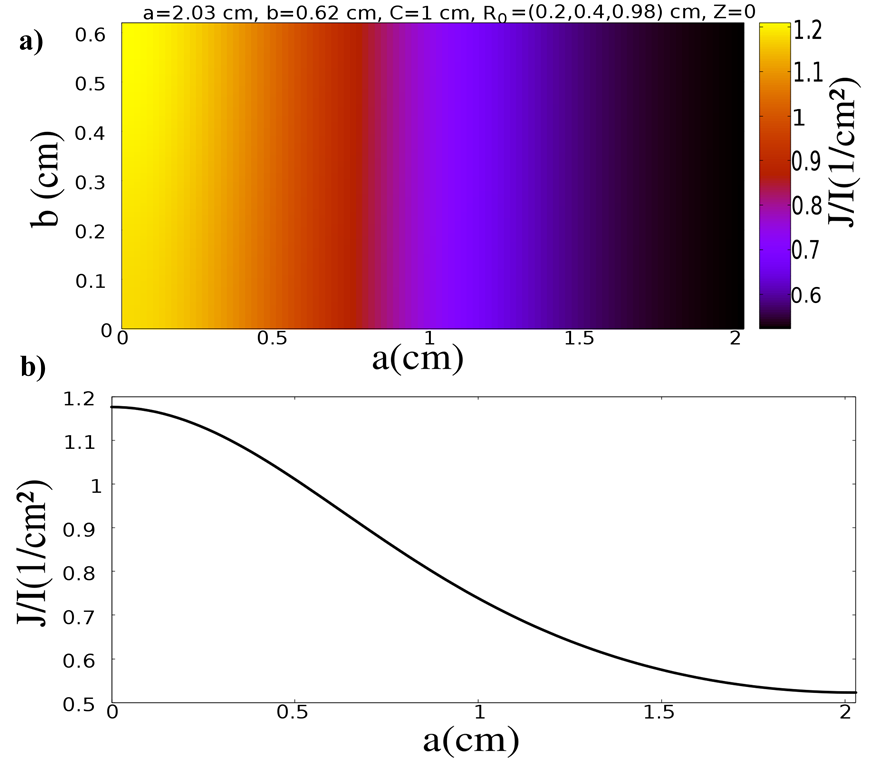
\includegraphics[scale=0.7]{Images/G123}
  \caption{\emph{ Simulation to calculate the current density in
      a structure with gradient refractive index (GRIN) produced
      by electrochemical attack on crystalline silicon to
      produce porous silicon (PS), with a current density
      profile $ J (mA / cm ^ 2 ) $ normalized with the electric
      current $ I (mA) $, we have $ J / I \sim 0.5 \ \ a \ \ 1.2
      (cm^{-2}) $, for a cell of $ a = 2.03 \ \ cm $ y $ b =
      0.62 \ \ cm $, with an electrode height $ Z_0 = 0.96 \ \
      cm $} Eq. (\ref{Eq:J})}.
  \label{fig:DR1}
\end{figure}
We consider Fig. \ref{fig:DR1} which come from solving
Eq. (\ref{Eq:J}), calculating the current density as a function of the
rectangular cell area of $1,206 \ \ cm^2 $,  the programming with the
PERL PDL package and corresponding graph in gnuplot. We optimize the
appropriate values so that our current density adequately attacks
crystalline silicon, giving the gradient effect. We use as length $a =
2.03 \ \ cm $ and width $b = 0.62 \ \ cm $ the height of the solution
is $ c = 1 \ \ cm $ and we could locate the tip of the electrode at $
R_0 = (X_0 = 0.2 , \ \ Y_0 = 0.4 \ \, Z_0 = 0.96) \ \ cm $ and
evaluated at the surface on the silicon interface, in the plane $ Z =
0 $. In this same Figure \ref{fig:DR1}, we obtain a current density
profile $ J (mA / cm^2) $ normalized with the electric current $ I
(mA) $, we have $ J / I \sim 1.2 \ \ a \ \ 0.5 (cm ^{-2}) $, as we see
in Fig. \ref{fig:DR1} a) an effect that happens on the surface of the
sample, a change of contrate due to the different densities of
attacked currents. We see the decay behavior that the profile has as
Fig. \ref{fig:DR1} b) which is a cut on the axis of $ a $. When we
vary the currents we can observe the behavior of changes in the
normalized current density, with the data obtained through the
simulation we could have a better optimization in the design of porous
silicon proposing a new and novel experimental arrangement, in the
same way we can give ourselves an idea by means of the graph of how
the attack would be and the formal side of the pores in the silicon.

\subsection{Monolayers GRIN Porous Silicon }
\begin{figure}
	\centering
	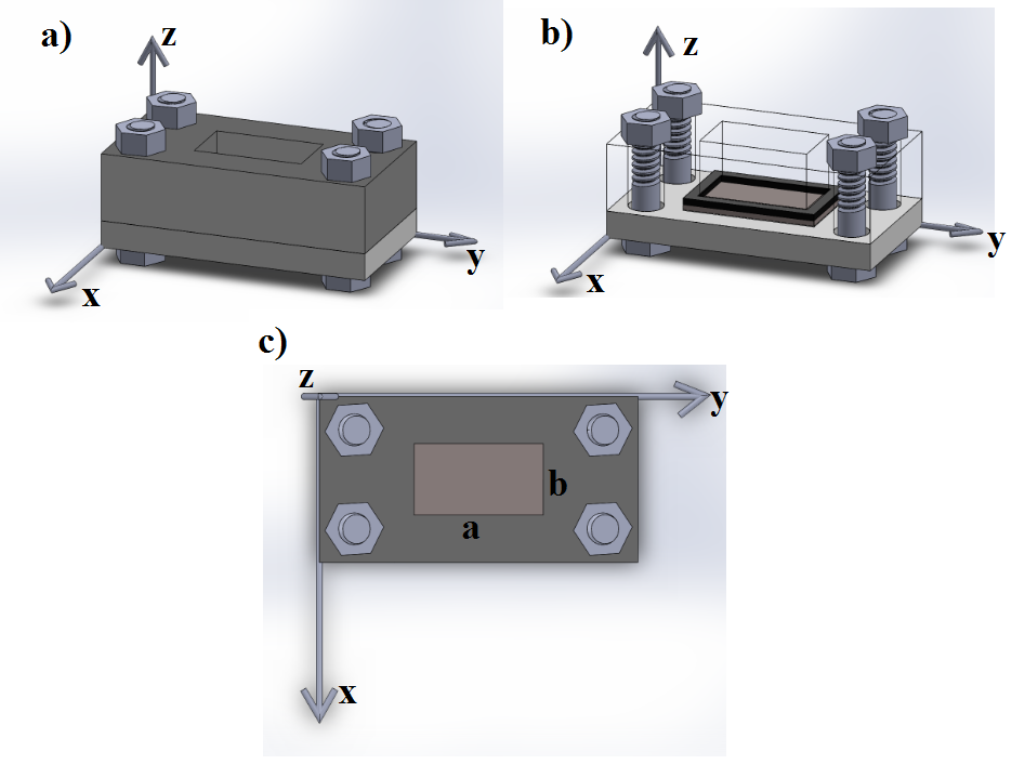
\includegraphics[scale=.3]{Images/celdan2}
	\caption{\emph{ Mechanical 3D modeling, design of the
            electrochemical cell where we can see the shape of a prism
            giving the required and necessary data for the
            experiments. The design of the cell used is $ 1,206 \ \ cm
            ^ 2 $ (this is the area attacked in the process), the area
            attacked is rectangular ($ 0.62 \ \ cm \times 2.03 \ \ cm
            $) and a height ( $ 1.2 \ \ cm $) a) Complete cell b) Cell
            without top cover and c) Top view}}
	\label{fig:por1}
\end{figure}
We can see in Fig. \ref{fig:por1}, 3D modeling the mechanical design
for the electrochemical cell  better optimization in manufacturing
silicon pores where we can see the shape of a prism giving the
required data. The design of the cell used is $ 1,206 \ \ cm ^ 2 $
(this is the area attacked in the process), the area attacked is
rectangular ($ 0.62 \ \ cm \times 2.03 \ \ cm $) and a height ( $ 1.2
\ \ cm $), all this in order to optimize our experiments adjusted to
all the needs that this required.
\begin{figure}
  \centering
  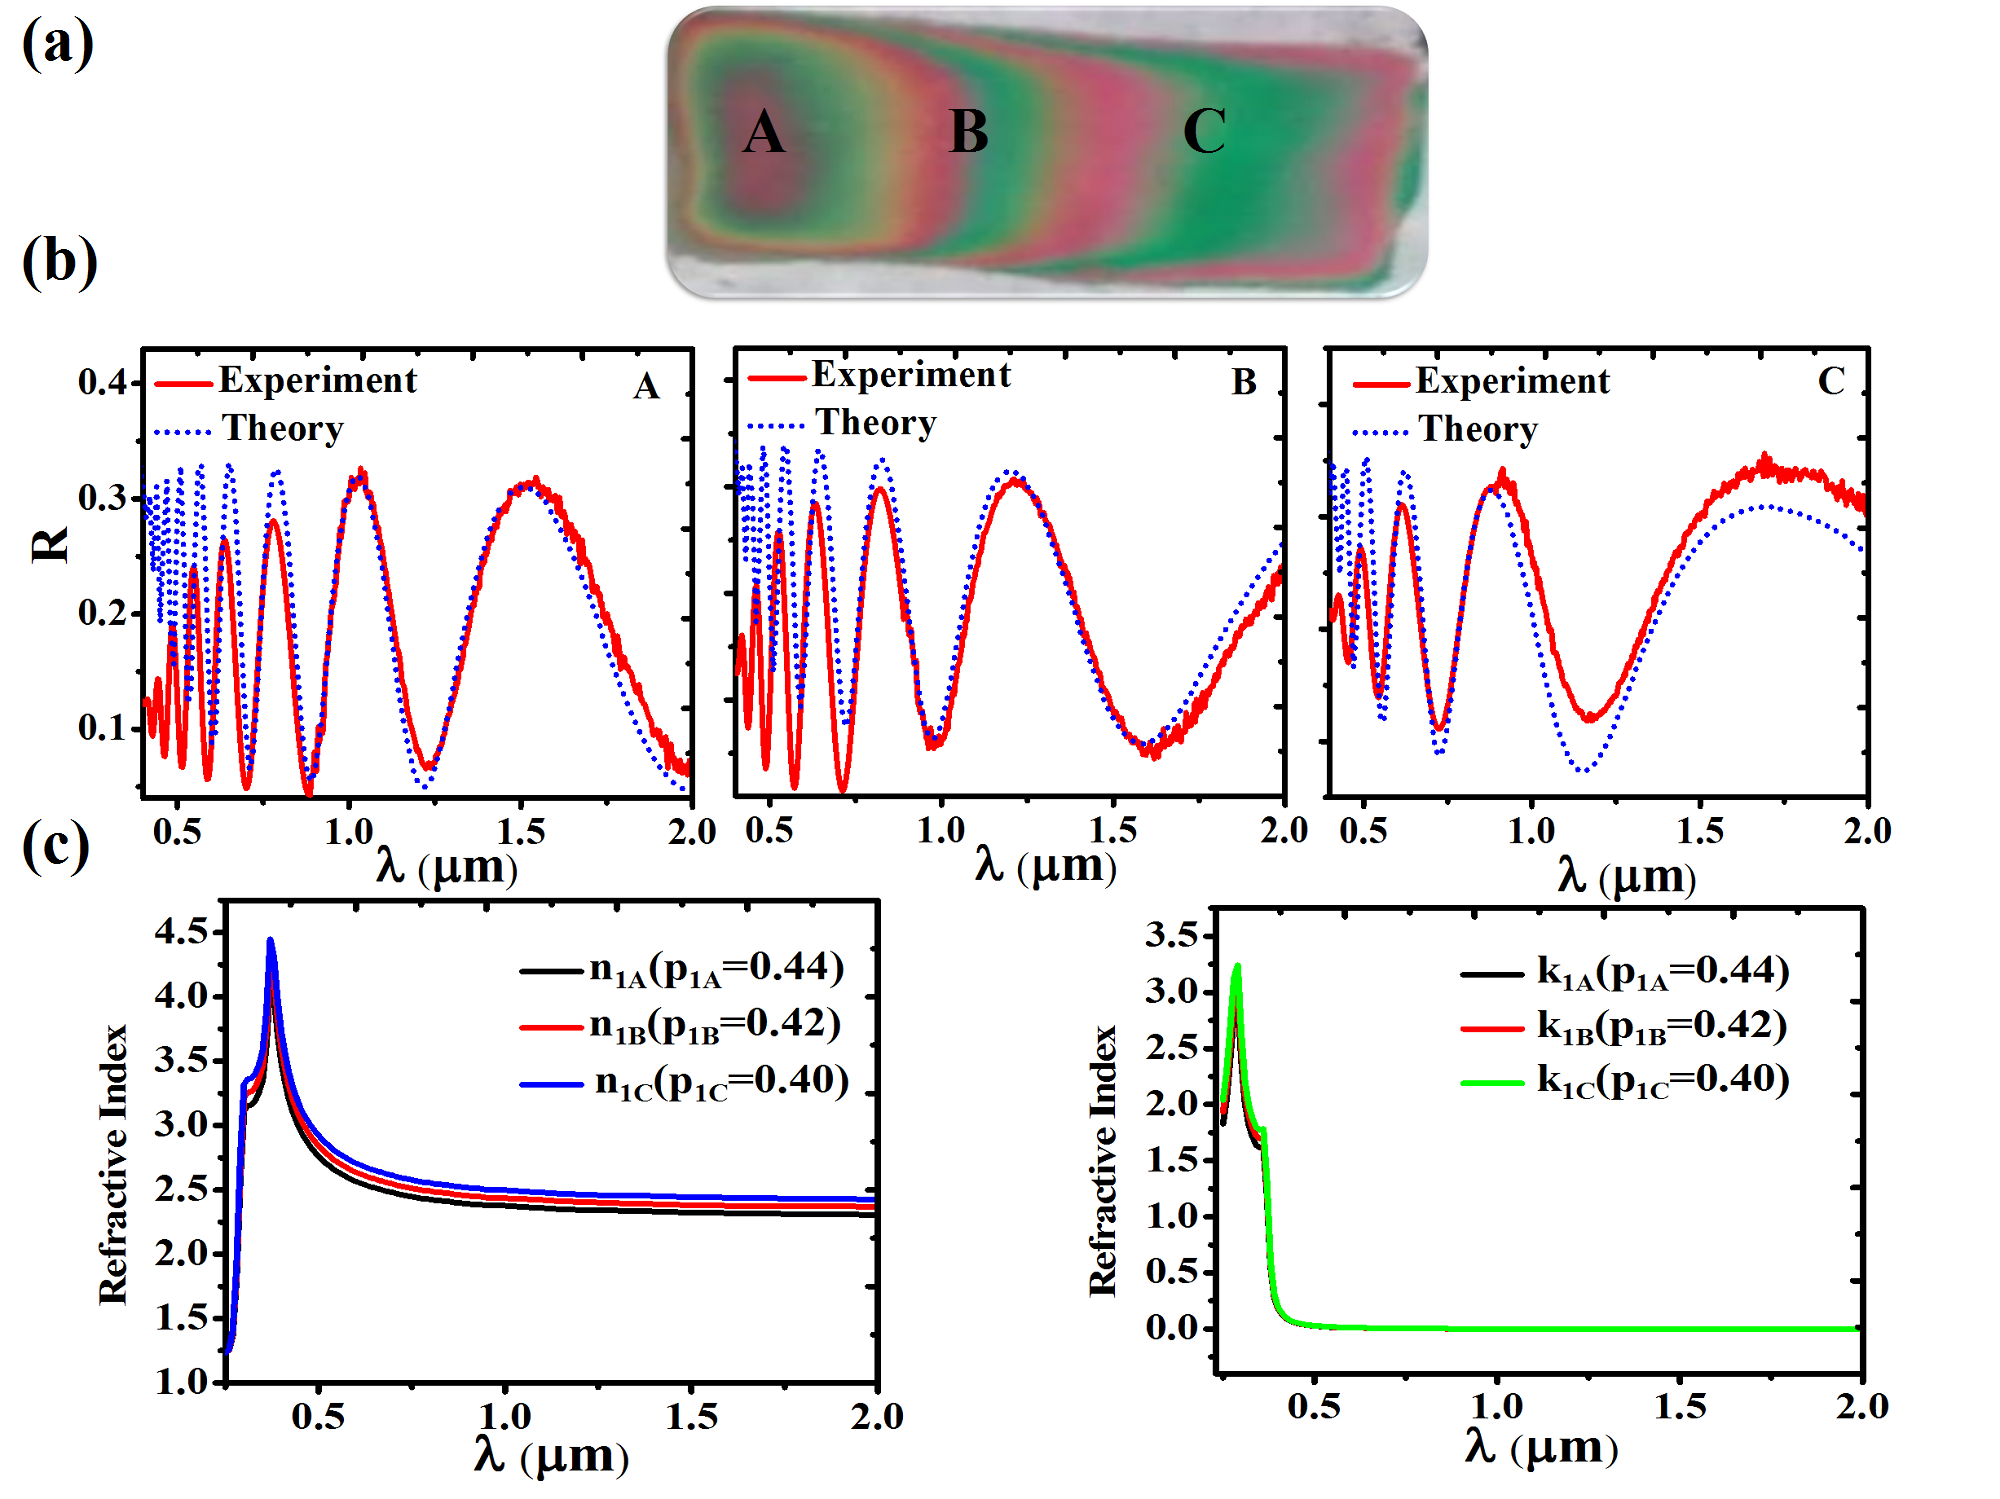
\includegraphics[scale=.5]{Images/SPgrin51}
  \caption{\emph{a) Silicon sample attacked with an electrolytic
      mixture of aqueous hydrofluoric acid (HF) (concentration:
      48 $ \% $  wt), glycerol (purity: 99.8 $ \% $  wt) and
      ethanol (purity: 99.9 $ \% $  wt ) in 3: 7: 1 volume
      ratio, respectively. Obtaining a monolayer of porous
      Silicon with GRIN G1 with an initial current of G1 (5 mA),
      with an attack time of 600s. Three different locations are
      considered, denoted as follows, A (0.3cm) and B (0.8cm)
      and C (1.7cm). b) Reflectance measurements to know the
      optical properties at each of the points and the
      adjustments that were produced by means of the equation
      \ref{Eq:ECMR}. c) We have the indices of refraction of the
      complex porous silicon GRIN, where we calculate the real
      and imaginary part by means of the equation
      \ref{Eq:Brugg}. for different porosities at each point, A
      (P = 0.44), B (P = 0.42) and C (P = 0.40) } }
  \label{fig:DR3}
\end{figure}
 The Fig. \ref{fig:DR3} a) three locations at different points are
 considered, denoted as follows, $ A (0.3 \ \ cm) $ and $ B (0.8 \ \
 cm) $ and $ C (1.7 \ \ cm) $, from the sample of PS GRIN $ G1 (I = 5
 mA) $. Also the Fig. \ref{fig:DR3}. b), we have the reflectance
 measurements to know the optical properties and the adjustments that
 were produced by means of the equation \ref{Eq:ECMR}. In the
 Fig. \ref{fig:DR3} c) are indices of refraction of the porous silicon
 complex GRIN, where we calculate the real and imaginary part by means
 of Eq. \ref{Eq:Brugg} for different porosities at each point, $ A (P
 = 0.44) $, $ B (P = 0.42) $ and $ C (P = 0.40) $. Location $ A $ is
 closest to the electrode, while location $ C $ is furthest to the
 other end of the sample. Since the current density is applied from
 one end, the field lines attack the sample laterally to the silicon
 wafer, in the present configuration, an assembly was made based on
 the simulated data shown in Fig. \ref{fig:DR1} the experimental part
 was taken a platinum electrode covering its surface, leaving only a
 very small area, as if it were a tip. The electrochemical reaction
 takes place when we apply currents from an anode end (electrode tip)
 to the silicon substrate (resistivity $ 0.002 - 0.005  \Omega \cdot
 cm $), through an electrolyte forming a current circuit. The
 reflectance spectra of the newly recorded G1 samples measured at
 points $ A (0.3 \ \ cm) $ and $ B (0.8 \ \ cm) $ and $ C (1.7 \ \ cm)
 $ are presented in Fig. \ref{fig:DR3} b), a numerical reflectivity
 adjustment was performed using the transfer matrix method for the
 case of a porous monolayer in Si. It should be noted that the
 adjustment made was considered a spectral range of the wavelength of
 the experimental reflectivity spectra for which the silicon can be
 considered the complex index and thus find the refractive index of
 the complex porous silicon with the purpose of determining the
 porosity and the experimental physical thickness (nm) by means of the
 SEM. The formation of PS GRIN in the thickness occurs due to the
 variation in the concentration of the voids available at the Si
 electrolyte interface, therefore, an increase in the applied lateral
 current density increases the dimension of the pores and their
 depth. Thus, the extent of the porous film showing a gradient that
 can be controlled from the lateral current density.
\begin{figure}
  \centering
  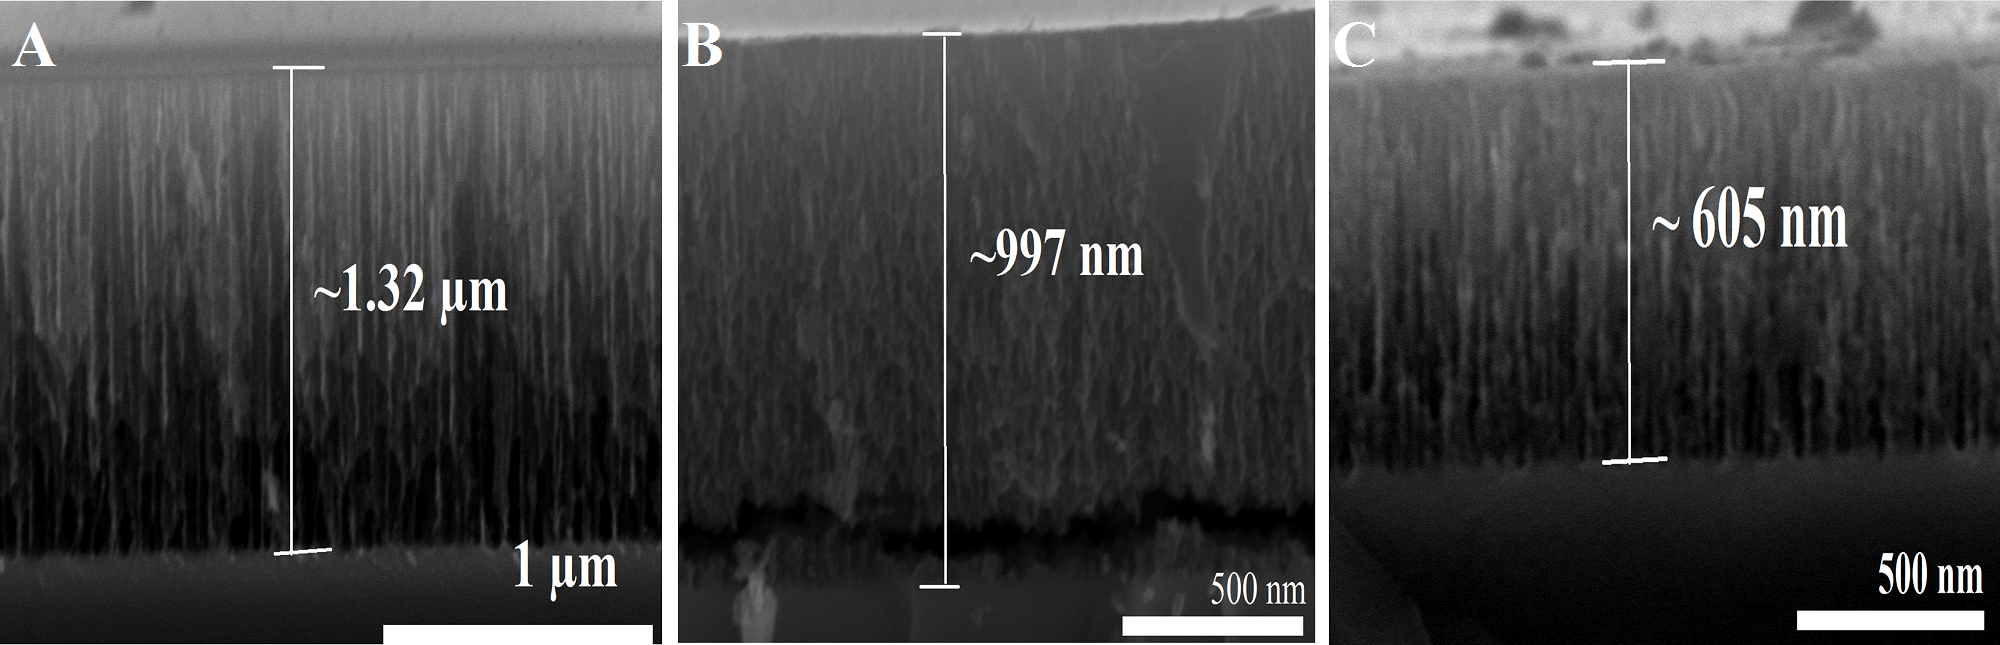
\includegraphics[scale=.5]{Images/semD11}
  \caption{\emph{Characterization of a monolayer of PS GRIN G1
      with an initial current of $ 5 \ \ mA $, seeing the
      morphology and depth of the cross section of several SEM
      micrographs, at different points, $ A (0.3 \ \ cm) $ and $
      B (0.8 \ \ cm) $ and $ C (1.7 \ \ cm) $. We can see the
      sample size for each measurement point, the depth $ d (A)
      = 1320 \ \ nm $, $ d (B) = 997 \ \ nm $ and $ d (C) = 605
      \ \ nm $ } }
  \label{fig:DR4}
\end{figure}
In the Fig. \ref{fig:DR4} shows the cross section views   at points $
A (0.3 \ \ cm) $, $ B (0.8 \ \ cm) $ and $ C (1.7 \ \ cm) $, we can
measure the thickness for each point of the sample $ G1 (I = 5 \ \ mA)
$, $ d (A) = 1320 \ \ nm $, $ d (B) = 997 \ \ nm $ and $ d (C) = 605 \
\ nm $. Likewise, we could check it for a second sample $ G2 (I = 40 \
\ mA) $, with porosities for each point, $ A (P = 0.76) $, $ B (P =
0.73) $ and $ C (P = 0.68) $ and the depths $ d (A) = 1950 \ \ nm $, $
d (B) = 1690 \ \ nm $ and $ d (C) = 1430 \ \ nm $, designed in the
same way as the shows G1, only varying the current taking into account
the current density ratio for each point. Apart from that, a
structural gradient was formed, along the direction \emph{ a}  of the
axis of the $ x $, where the tip of the electrode is near the point $
A $ and away from the point $ C $ of the substrate, using the proposed
experimental setup. In addition, it was possible to control the
current density based on the position of the sample and the depth,
seen in the SEM micrographs.
 \begin{figure}
   \centering
   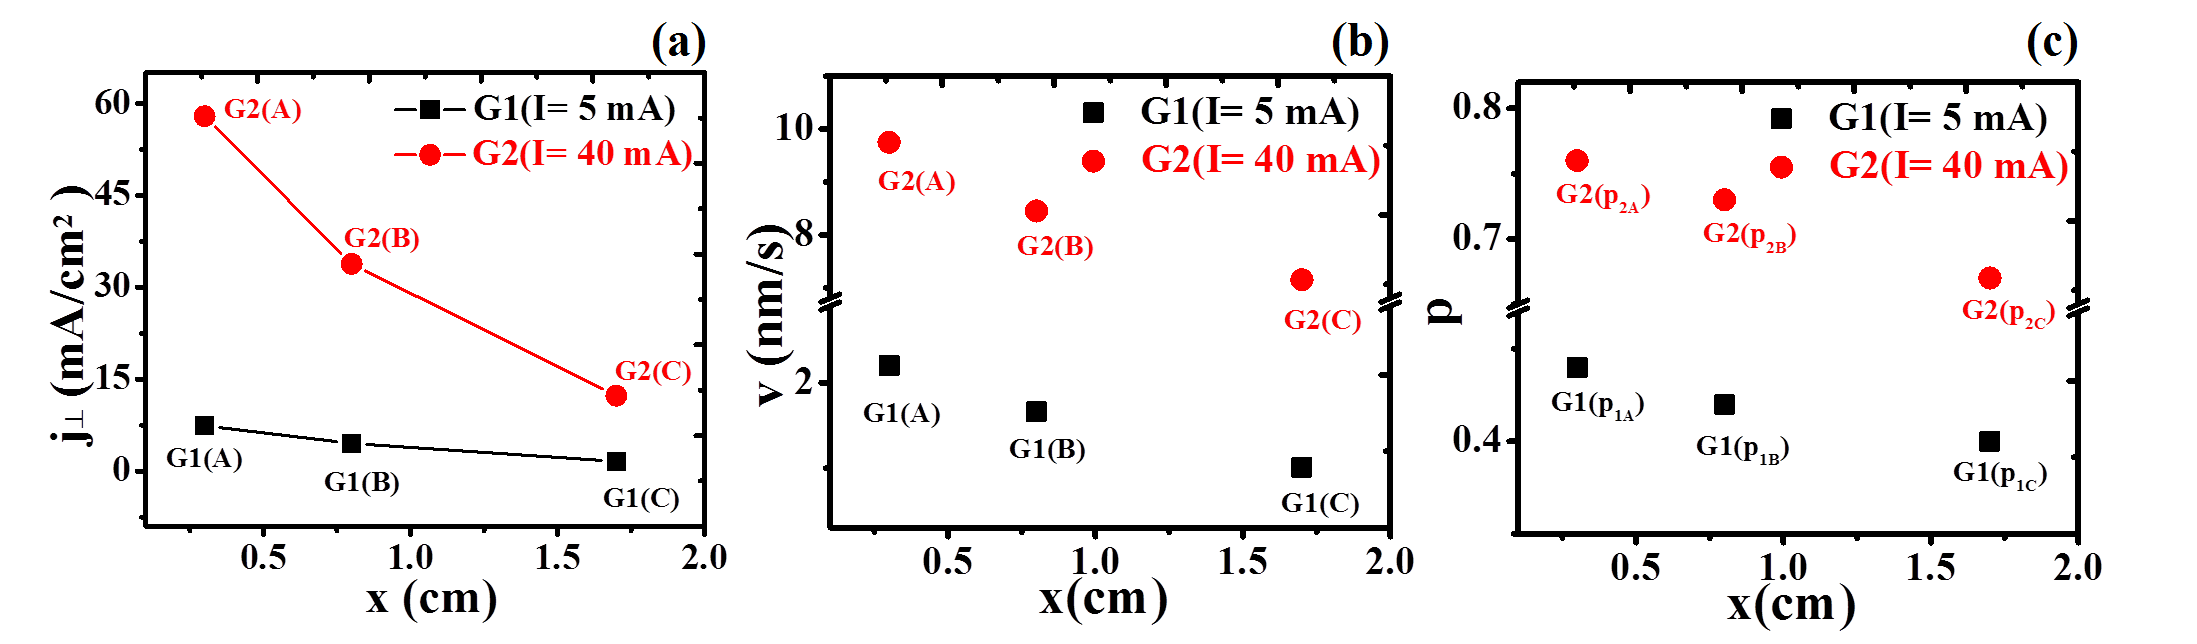
\includegraphics[scale=.7]{Images/grinJDR}
   \caption{\emph{a) It is the relation of the current density $
       J (mA / cm ^ 2) $ normalized with the electric current $ I
       (mA) $, we have $ J / I \ sim 1.2 \ \ a \ \ 0.5 ( cm^{-2})
       $, when we apply it to two samples $ G1 (I = 5 \ \ mA) $
       and $ G2 (I = 40 \ \ mA) $ depending on the axis $ a $ $
       (0.1 ... 2.0 \ \ cm) $, measured at points $ A (0.3 \ \
       cm) $ , $ B (0.8 \ \ cm) $ and $ C (1.7 \ \ cm) $. b) The
       attack speed $ v = d (J_i) / t (nm / sec) $, the depths
       (thickness $ d (J_i) $, $ i = $ $ A (0.3 \ \ cm) $, $ B (
       0.8 \ \ cm) $ y $ C (1.7 \ \ cm)) $ taken in SEM
       micrographs $ d (J_i) (nm) $ and attack times $ G1 (t =
       600 \ \ s) $ y $ G2 (t = 200 \ \ s) $, depending on the
       axis $ a $ $ (0.1 ... 2.0 \ \ cm) $ } }
   \label{fig:JDR}
 \end{figure}
In Fig. \ref{fig:JDR} a) It is the relation of the current density $ J
(mA / cm ^ 2) $ normalized with the electric current $ I (mA) $, we
have $ J / I \ sim 1.2 \ \ a \ \ 0.5 (1 / cm ^ 2) $, when we apply it
to two samples $ G1 (I = 5 \ \ mA) $ and $ G2 (I = 40 \ \ mA) $
depending on the axis $ a $ $ (0.1 ... 2.0 \ \ cm) $, measured at
points $ A (0.3 \ \ cm) $ and $ B (0.8 \ \ cm) $ and $ C (1.7 \ \ cm)
$.
The Fig. \ref{fig:JDR} b) we can calculate the attack speed $ v = d
(J_i) / t (nm / s) $, where the depths (thickness $ d (J_i) $, $ i = $
$ A (0.3 \ \ cm) $, $ B (0.8 \ \ cm) $ and $ C (1.7 \ \ cm)) $ taken
in SEM micrographs $ d (J_i) (nm) $ and attack times $ G1 (t = 600 \ \
s) $ and $ G2 (t = 200 \ \ s) $, depending on the axis $ a $ $ (0.1
... 2.0 \ \ cm) $.
\begin{figure}
  \centering
  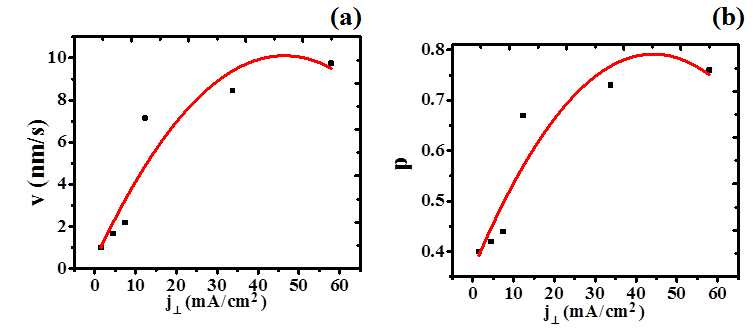
\includegraphics[scale=.6]{Images/grinJD31}
  \caption{\emph{The relationship of samples $ G1 (I = 5 mA) $ and $
      G2 (I = 40 mA) $ were obtained to find: a) Attack speed with
      current density for each point and b) Porosity as a function of
      density current. With this we have the calibration curves for
      the manufacture of any GRIN porous silicon structure   } }
  \label{fig:Indr1}
\end{figure}
Fig. \ref{fig:Indr1} a) explicitly explain the relationships that
emerge when designing samples $ G1 (I = 5 mA) $ and $ G2 (I = 40 mA)
$. For the first case $ G1 $ the depths ($ 1320 \ \ nm $ to $ 605 \ \
nm $) and the current densities ($ 6 \ \ mA / cm ^ 2 $ to $ 2.5 \ \ mA
/ cm ^ 2 $), finding the attack speed $ 2.2 \ \ nm / s $ up to $ 1.1 \
\ nm / s $ relation with depth and the time ($ 600 \ \ s $) of
exposure of the sample, with the current density . We also find the
depth ($ 1950 \ \ nm $ at $ 1430 \ \ nm $) and the current density ($
50 \ \ mA / cm ^ 2 $ at $ 20 \ \ mA / cm ^ 2 $) as a function of the
measurement points of the sample $ G2 (I = 40 mA) $. We were able to
obtain the attack speed from $ 9.8 \ \ nm / s $ up to $ 7.1 \ \ m / s
$ by relating to depth and time ($ 200 \ \ s $), with current
density. Once the thickness of the monolayer and the attack time
applied to them are known, calculate the attack speed according to the
formula $ v = d / t $, for each of the current densities at the points
$ A ( 0.3 \ \ cm) $ and $ B (0.8 \ \ cm) $ and $ C (1.7 \ \ cm)
$. Then we fit a function to the attack speed points with the
different current densities allowed by the anodizing condition. For a
desired thickness $ d (J_i) $, calculate the attack time $ t $ (so, $
t = v / d (J_i) $) and we can design any structure knowing the current
density and the attack time. Fig. \ref{fig:Indr1} b) we find a
relation of the porosity for each position with its determined current
density. Therefore, if it is desired to manufacture a PS monolayer of
a certain porosity with a certain end, it is enough to resort to the
graphs of Fig. \ref{fig:Indr1} to determine the corresponding current
density, attack speed and consequently the time, obtaining for that
monolayer. The importance of the calibration curves is that it allows
us to have a relationship of the porosities that can be reached (and
by having control over the possible refractive indices) as a function
of the current density and to be controlled to control the thickness
of the layers that are manufactured, by controlling the attack time
for each of the chosen currents.

\subsection{GRIN Porous Silicon Microcavities}
 \begin{figure}
	\centering
	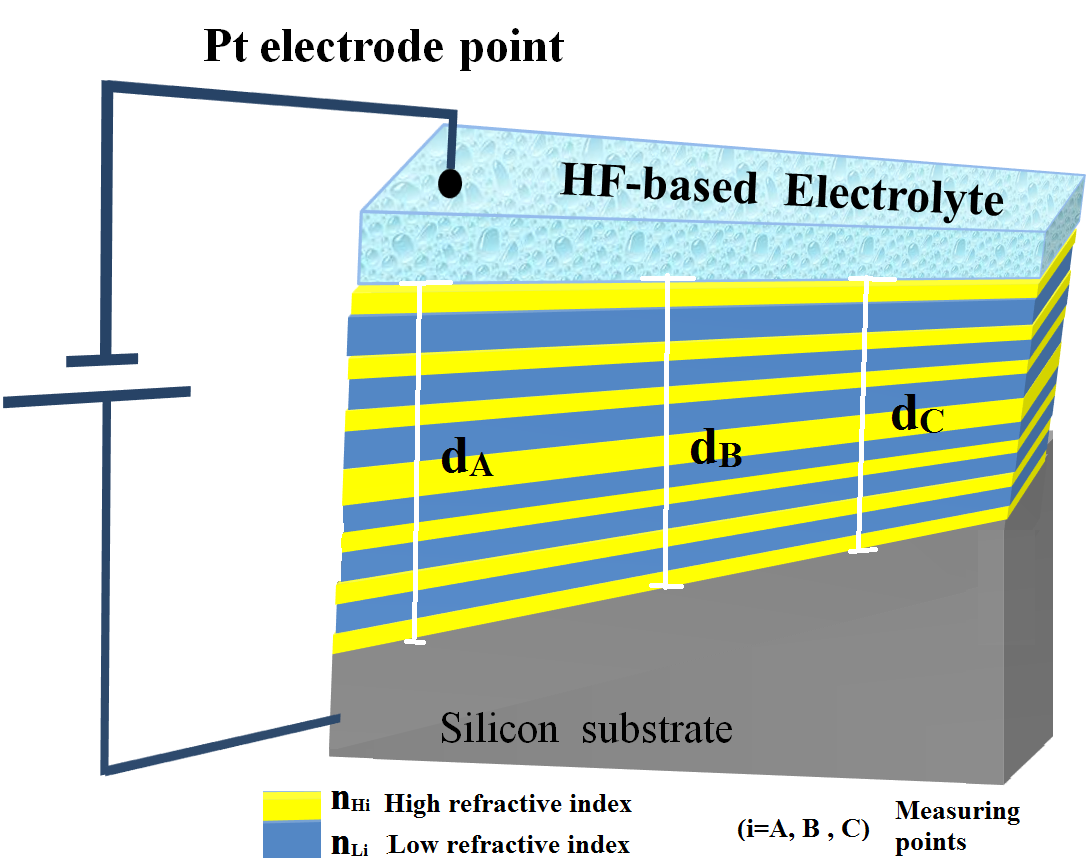
\includegraphics[scale=0.4]{Images/MicrGrin}
	\caption{\emph{Diagram of a microcavity of porous silicon
            GRIN. Alternate layers are obtained of high (H) refractive
            index $n_{_{Hi}}$ and low (L) refractive index
            $n_{_{Li}}$, where $N_{_{H}}$ is the number of layers for
            $n_{_{Hi}}$ and $N_{_{L}}$ is the number of layers for
            $n_{_{Li}}$. Then,  $d_{_{Hi}}$ is the monolayer thickness
            of  $n_{_{Hi}}$ at that measurement point and $d_{_{Li}}$
            is the monolayer thickness of $n_{_{Hi}}$ at that
            measurement point. Therefore,  $d_{_{i}}$ is the total
            thickness calculated for each of the measurements,
            defining a i = $ A, B, C$. Having the following
            relationship $d_{_{i}} =
            (N_{_{Hi}}d_{_{Hi}})+(N_{_{Li}}d_{_{Li}}) +
            (2d_{_{Hi}})$. }}
	\label{fig:MCGRIN0}
\end{figure}
The Fig. \ref{fig:MCGRIN0} the scheme of  a initially proposed lateral
gradient for monolayers should be shown in section 4.2, where we
designed an electolytic cell suitable for our experiments and giving
us the expected results of the simulation in section 4.1. Now our
purpose is to manufacture more complex photonic structures such as the
Porous silicon microcavities GRIN, taking into account that we start
from having a tip electrode almost on the surface and by making a
variation of currents we can achieve the effect of alternating the
layers. Alternate layers are obtained of high (H) refractive index
$n_{_{Hi}}$ and low (L) refractive index $n_{_{Li}}$, where $N_{_{H}}$
is the number of layers for  $n_{_{Hi}}$ and $N_{_{L}}$ is the number
of layers for $n_{_{Li}}$. Then,  $d_{_{Hi}}$ is the monolayer
thickness of  $n_{_{Hi}}$ at that measurement point and $d_{_{Li}}$ is
the monolayer thickness of $n_{_{Hi}}$ at that measurement
point. Therefore,  $d_{_{i}}$ is the total thickness calculated for
each of the measurements, defining a i = $ A, B, C$. Having the
following relationship $d_{_{i}} =
(N_{_{Hi}}d_{_{Hi}})+(N_{_{Li}}d_{_{Li}}) + (2d_{_{Hi}})$.
Initial data for conventional design we use  $\lambda_{_{c}}= 0.67 \ \
\mu m$, $n_{_{H}} =2.6$, $P_{_{H}} =0.46$, $d_{_{H}}=0.066 \ \ \mu m
$, $t_{_{H}}=35 s  $ y para  $n_{_{L}}= 1.4$,  $P_{_{L}} =0.75$,
$d_{_{L}}=0.117 \ \ \mu m  $, $t_{_{L}}=11 s  $. All these data are
for the point $ 0 $ which is located at one end of the sample just
below the tip counter-electrode.
\begin{figure}
  \centering
  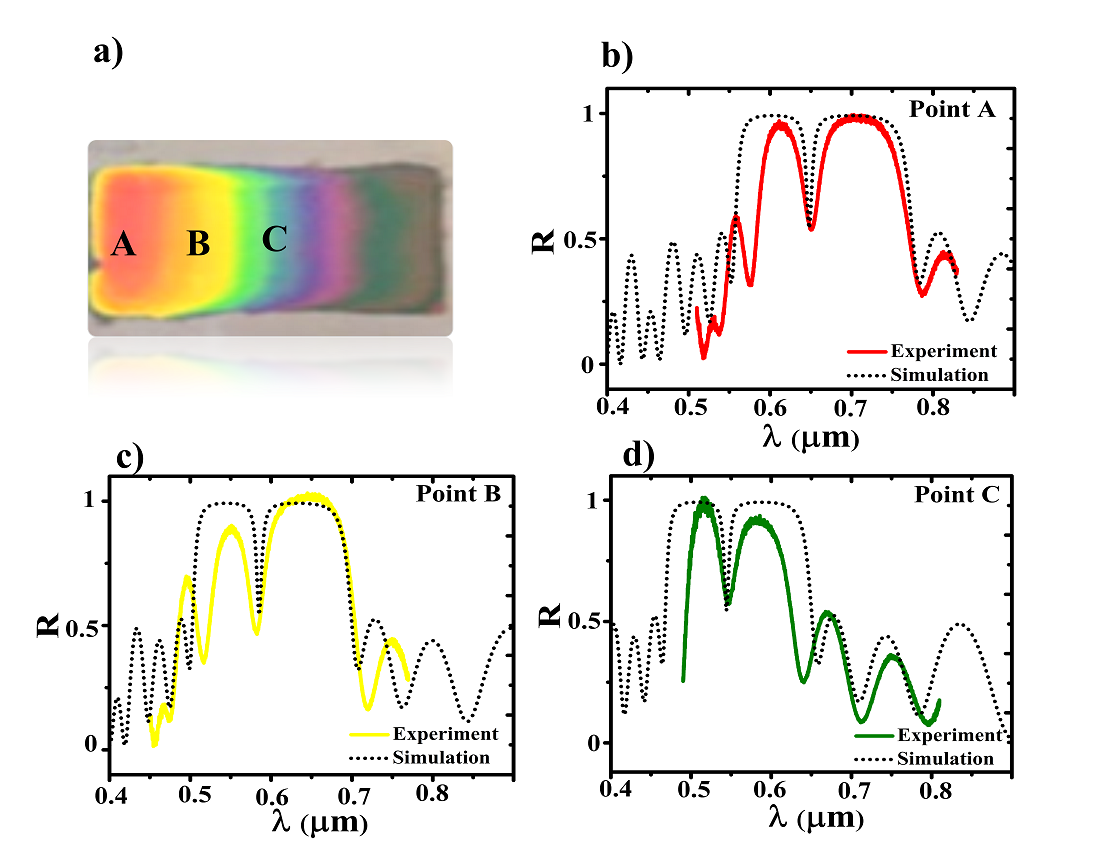
\includegraphics[scale=.5]{Images/MCGRIN2}
  \caption{\emph{a) Three locations at different points are
      considered, denoted as follows, $ A (0.3 \ \ cm) $ and $ B
      (0.8 \ \ cm) $ and $ C (1.2 \ \ cm) $, from the PSMCGRIN
      sample $ GMC $. b) We have the reflectance measurements to
      know the optical properties with the proposed
      simulation. We were able to show that in a Porous Silicon
      GRIN structure, for a microcavity the data is very
      consistent with the simulation and the experiment, we
      found the refractive indices and the porosities as a
      function of the current density at each measurement point,
      see Table \ref{tabla:1}. }}
  \label{fig:MCGRIN3}
\end{figure}

\begin{table}
  \centering
  \begin{tabular}{|c|c|c|c|c|c|c|}
    \hline
    \textbf{Points} & $\lambda_c (\mu m)$ & \textbf{n} & \textbf{k} & \textbf{Porosity} & \textbf{J}$(mA/cm^2)$ & \textbf{t(s)}\\
    \hline
    A(H) & 0.65 & 2.661 & 0.0264 & 0.45 & 5.5 & 35 \\
    \hline
    B(H) & 0.58 & 2.762 & 0.0135 & 0.41 & 4.0 & 35 \\
    \hline
    C(H) & 0.54 & 2.808 & 0.0178 & 0.39 & 3.0 & 35 \\
    \hline
    A(L) & 0.65 & 1.442 & 0.0015 & 0.74 & 44 & 11 \\
    \hline
    B(L) & 0.58 & 2.295 & 0.0091 & 0.68 & 32 & 11 \\
    \hline
    C(L) & 0.54 & 2.302 & 0.001 & 0.64 & 24 & 11 \\
    \hline
  \end{tabular}
  \caption{ \emph{We have different points denoted as follows, $ A
      (0.3 \ \ cm) $ and $ B (0.8 \ \ cm) $ and $ C (1.2 \ \ cm) $,
      from the sample of a Porous Silicon Microcavity GRIN
      (PSMCGRIN) $ GMC $. Alternate layers of high refractive index
      (H) and low refractive index (L) are obtained at each of the
      measurement points (A, B and C). The refractive indexes of the
      PSMCGRIN were considered from the experimental and theoretical
      values that were obtained for the porosity ($ P =
      0.3J^{0.24}$). And we could obtain the attack time with the
      relation of $ V = 0.53J ^ {0.79} $ where $ t = d / V $.}}
	\label{tabla:1}
\end{table}
In Fig. \ref{fig:MCGRIN3} a) Three locations at different points are
considered, denoted as follows, $ A (0.3 \ \ cm) $ , $ B (0.8 \ \ cm)
$ and $ C (1.2 \ \ cm) $, from the PSMCGRIN sample $ GMC $. Likewise,
Fig. \ref{fig:DR3} b), we have the reflectance measurements to know
the optical properties with the proposed simulation. We can see how
from an experimental setup we have some important results as a result
of a whole calibration curve suitable for making GRIN porous
silicon. The refractive index of the Porous Silicon Microcavities GRIN
were considered the experimental and theoretical values obtained for
the porosity and the thicknesses shown in Table 1. The porous silicon
microcavities (MCSP) with refractive index with gradient (GRIN), were
manufactured with different current densities ranging from $ 6 \ \ mA
/ cm ^ 2 $ to $ 2.5 \ \ mA / cm ^ 2 $ for a current of $ 5 \ \ mA $,
for a $t_{_{H}}=35 s $, with a high refractive index $n_{_{H}} \sim$ $
2,661$ to $ 2,808$ and porosities of $P_{_{H}} \sim$ $ 0.45 $ to $
0.39 $. Also for $ 44 \ \ mA /cm^2 $ to $ 24 \ \ mA / cm^2 $, current
of $ 38 \ \ mA $, using $t_{_{H}}=11 s$  for low refractive index
$n_{_{L}}\sim$ $ 1,448 $ to $ 2,267 $ and with porosities of
$P_{_{H}} \sim$ $0.75 $ to $ 0.64 $. The porosity was calculated with
the calibration curve exposed in the ($ P = 0.3J^{0.24} $). And the
attack time could be obtained with the relation of $ V = 0.53J^{0.79}
$ where $ t = d / V $ and the refractive index using the Bruggeman
formula. For theoretical values, we use complex refractive indices as
free parameters to fit the experimental refractive spectra (Section
4.2).
 \begin{figure}
   \centering
   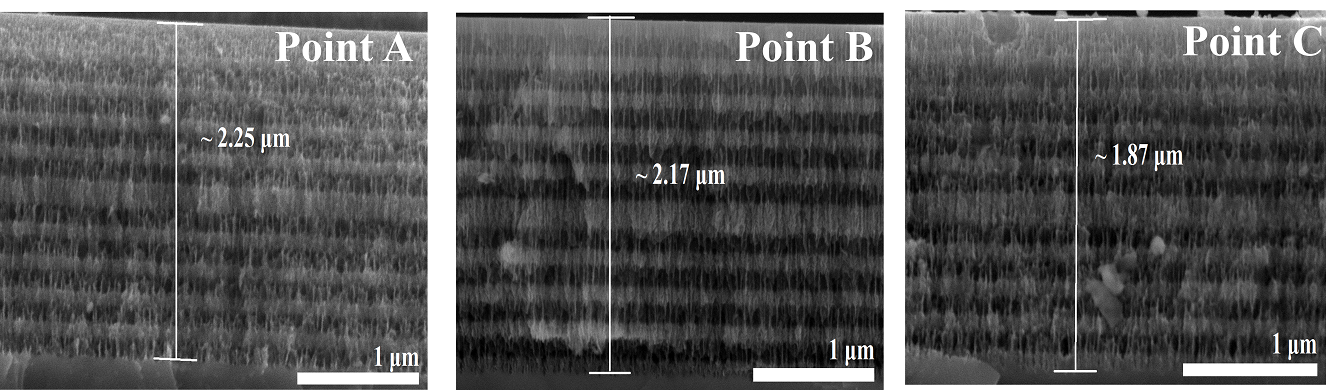
\includegraphics[scale=.5]{Images/MCGRINSEM}
   \caption{\emph{SEM image of the cross section profile of the
       microcavities with GRIN. The measured thicknesses of the
       complete multi-film structures showed good agreement with the
       simulations taken from $ V = 0.53J ^ {0.79} $ where $d_j=Vt_j$
       ($j=H,L$), which are the thicknesses of each of the monolayer
       of the porous silicon microcavity GRIN at the measurement
       points and the total thickness we find it as $d_{_{i}} =
       (N_{_{Hi}}d_{_{Hi}})+(N_{_{Li}}d_{_{Li}}) + (2d_{_{Hi}})$
       defining $ i = $ A, B, C. Which resulted in (measured /
       simulation) $ 2.25 / 2.31 \ \ \mu m $ (for structure at Point
       A), $ 2.17 / 2.08 \ \ \mu m $ (for structure at point B) and $
       1.87 / 1.65 \ \ \mu m $ (for structure at point C)}}
	\label{fig:MCGRIN4}
\end{figure}

For the Fig. \ref{fig:MCGRIN4} shows the SEM cross-sectional images of
the PS samples used in this work. Relatively small interface
roughness and a clear contrast between the high and low porosity of
the microcavity measured at different points (A, B and C), showing the
change in thickness in each of these. The measured thicknesses of the
complete multi-film structures showed good agreement with the
simulations taken from $ V = 0.53J^{0.79} $ where $d_j=Vt_j$
($j=H,L$), which are the thicknesses of each of the monolayer of the
porous silicon microcavity GRIN at the measurement points and the
total thickness we find it as $d_{_{i}} =
(N_{_{Hi}}d_{_{Hi}})+(N_{_{Li}}d_{_{Li}}) + (2d_{_{Hi}})$ defining $ i
= $ A, B, C. Which resulted in (measured / simulation) $ 2.25 / 2.31 \
\ \mu m $ (for structure at Point A), $ 2.17 / 2.08 \ \ \mu m $ (for
structure at point B) and $ 1.87 / 1.65 \ \ \mu m $ (for structure at
point C).
Being able to say that for each measurement point corresponds
different calculated current densities, which correspond to different
thicknesses at the end of manufacturing, clearly seeing the lateral
gradient product of our experiment.


\section{conclusion}
The necessary expressions for the potential components were derived,
finding a relationship of the tip of the counter electrode that acts
similarly as a point charge and the current density for a geometry in
a rectangular electrolytic box and we solve the electrostatic
equations with suitable boundary conditions. Resulting in an
electrostatic model for  Photonics crystals with a refractive index
with gradient (EMPCGRIN).
It is the first time that the formalism mentioned here has been
applied to find the current density to design porous silicon. The
shape of the electrode, the area of the cell produces a visible
decrease in the size and density of the pores. Additionally,
optimizing the structural properties for a single structure we could
have a gradient with different depths, reflactances at differents
measurement points. In this way, we were able to simulate the direct
relationship of the attack speed with the current density at the
points  the samples of interest. At the same time, we developed a
characterization between porosity, refractive indices of porous
silicon, with the different current densities. And in the end we were
able to design and characterize Porous Silicon microcavities with
refractive indices with gradients, which for each measurement point
correspond to different calculated current densities, which correspond
to different thicknesses, clearly seeing the lateral gradient product
of our experiment.
\section{Acknowledgments}
% \backmatter
%\nocite{*}
%\bibliographystyle{plain}
%\bibliography{bibliografía.bib} %Aquí ponen el nombre del archivo .bib
\bibliographystyle{unsrt}
\begin{thebibliography}{X}
  % forma de biblio es MLA
\bibitem{I1} P. Yeh,\textquotedblleft \emph{Optical Waves in Layered
    Media} \textquotedblright, 2nd edn. (Wiley-Interscience
  Publication,
  USA, 2005).
\bibitem{I2}Canham, L. 1997.\textquotedblleft \emph{Properties of
    Porous Silicon} \textquotedblright. Edited by Canham L. DERA,
  Malvern, UK.
\bibitem{I3}{Beale, M.I.J, J.D Benjamin, M.J Uren, N.G Chew, and A.G
    Cullis. 1985. \emph{ \textquotedblleft An Experimental and
      Theoretical Study of the Formation and Microstructure of
      Porous Silicon.\textquotedblright} J. Crystal Growth 73:
    622?36. doi:10.1021/jp0706984. }
\bibitem{I4}Canham, L. T. 1990. \emph{\textquotedblleft Silicon
    Quantum Wire Array Fabrication by Electrochemical and Chemical
    Dissolution of Wafers.\textquotedblright} Applied Physics
  Letters 57 (10): 1046. doi:10.1063/1.103561.
\bibitem{I5} J. D. Joannopoulos et al.,\textquotedblleft
  \emph{Photonic Crystals: Molding the Flow of
    Light}\textquotedblright, 2nd edn.
  (Princeton University Press, UK, 2008).
\bibitem{I6} E. Yablonovitch, \textquotedblleft \emph{Photonic
    band-gap structures,}\textquotedblright J. Opt. Soc. Am. B 10,
  283-295 (1993)
\bibitem{I7} Ilyas, S., and M. Gal.  \textquotedblleft \emph{
    Optical devices from porous silicon having continuously varying
    refractive index.}\textquotedblright Journal of Materials
  Science: Materials in Electronics 18.1 (2007): 61-64.
\bibitem{I8} Tran, P. \textquotedblleft \emph{Optical switching with
    a nonlinear photonic crystal: a numerical
    study.}\textquotedblright Optics letters 21.15 (1996):
  1138-1140.
\bibitem{I9} Ariza-Flores, A. David, L. M. Gaggero-Sager, and
  V. Agarwal. \textquotedblleft \emph{White metal-like
    omnidirectional mirror from porous silicon dielectric
    multilayers.}\textquotedblright Applied Physics Letters 101.3
  (2012): 031119.
\bibitem{I10} Johnson, Steven G., et al.  \textquotedblleft
  \emph{Linear waveguides in photonic-crystal
    slabs.}\textquotedblright Physical Review B 62.12 (2000): 8212.

  % asimetrica
\bibitem{I101}Collins, Boyce E., et al. \textquotedblleft \emph{
    Determining protein size using an electrochemically machined
    pore gradient in silicon.}\textquotedblright Advanced Functional
  Materials 12.3 (2002): 187-191.

\bibitem{I102} Khung, Y. L., G. Barritt, and
  N. H. Voelcker. \textquotedblleft \emph{Using continuous porous
    silicon gradients to study the influence of surface topography
    on the behaviour of neuroblastoma cells.}\textquotedblright
  Experimental cell research 314.4 (2008): 789-800.

\bibitem{I103} Clements, Lauren R., et al. \textquotedblleft
  \emph{Mesenchymal stem cell attachment to peptide density
    gradients on porous silicon generated by
    electrografting.}\textquotedblright physica status solidi (a)
  208.6 (2011): 1440-1445.

\bibitem{I104} Wang, Peng-Yuan, et al. \textquotedblleft
  \emph{Screening the attachment and spreading of bone
    marrow-derived and adipose-derived mesenchymal stem cells on
    porous silicon gradients.}\textquotedblright Rsc Advances 2.33
  (2012): 12857-12865.
\bibitem{I11} Canham, L. \textquotedblleft \emph{Properties of
    Porous Silicon.}\textquotedblright Edited by Canham L. DERA,
  Malvern, UK. (1997).
\bibitem{I12} Li, Yang Yang, Peter Kim, and Michael J
  Sailor.\textquotedblleft \emph{Painting a Rainbow on Silicon A
    Simple Method to Generate a Porous Silicon Band Filter
    Gradient}\textquotedblright Physica Status Solidi (a) 1618 (8):
  161618. doi:10.1002/pssa.200461200.(2005)
\bibitem{I13} Khung, Y L, and N H
  Voelcker. 2009.\textquotedblleft\emph{ Multidirectional Lateral
    Gradient Films with Position-Dependent Photonic Signatures Made
    from Porous Silicon.}\textquotedblright Optical Materials 32
  (1): 23442. doi:10.1016/j.optmat.2009.07.015.
\bibitem{I14}  Khung, Y L, G Barritt, and N H Voelcker.
  \textquotedblleft \emph{Using Continuous Porous Silicon Gradients
    to Study the Influence of Surface Topography on the Behaviour of
    Neuroblastoma Cells.}\textquotedblright Experimental Cell
  Research 314 (4): 78900. doi:10.1016/j.yexcr.2007.10.015.(2008.)
\bibitem{I15} Collins, B.E., K.-P.S. Dancil, G. Abbi, and
  M.J. Sailor. 2002.\textquotedblleft \emph{Determining Protein Size
    Using an Electrochemically Machined Pore Gradient in
    Silicon.}\textquotedblright Advanced Functional Materials 12 (3):
  187. doi:10.1002/1616-3028(200203)12:3,187::AID-ADFM187,3.0.CO;2-E.(
  2002.)

\bibitem{I16} Ocier, C. R., Krueger, N. A., Zhou, W. and  Braun,
  P. V. (2017).\textquotedblleft \emph{Tunable visibly transparent
    optics derived from porous silicon.}\textquotedblright ACS
  Photonics, 4(4), 909-914.
\bibitem{I17} Dariani RS, Ebrahimnasab S (2014). \textquotedblleft
  \emph{Root Mean Square Roughness of Nano Porous Silicon by
    Scattering Spectra.}\textquotedblright The
  European Physical Journal Plus 129: 129.
\bibitem{I18} Lerondel G, Romestain R (1997).\textquotedblleft
  \emph{Roughness of the Porous Silicon Dissolution
    Interface.}\textquotedblright Journal of Applied Physics 81:
  61716178.
\bibitem{I19} Lérondel G, Romestain R, Barret S
  (1997).\textquotedblleft \emph{Quantitative Analysis of the Light
    Scattering Effect on Porous Silicon
    Optical Measurements.}\textquotedblright Thin Solid Films 297:
  114?117.

\bibitem{I20} Thei, W. \textquotedblleft \emph{Optical Properties of porous silicon.}\textquotedblright Surf. Sci. Rep. 1997, 29, 91?93.
\bibitem{I21} Van Groesen, E.; Sopaheluwakan, A.; Andonowati,
  A. \textquotedblleft  \emph{Direct characterization of states and
    modes in defect grating structures.}\textquotedblright
  J. Nonlinear Opt. Phys. Mater. 2004, 13, 155173.

\bibitem{In} Mazzoleni, C., and L. Pavesi. \textquotedblleft
  \emph{Application to optical components of dielectric porous silicon
    multilayers.}\textquotedblright Applied Physics Letters 67.20
  (1995): 2983-2985

\end{thebibliography}

\end{document}